\documentclass[
    % english, % Klasei padavus parametrą 'english', darbas bus anglų kalba.
    % signatureplaces % prideda parašų vietas tituliniame puslapyje
]{VUMIFPSbakalaurinis}
\usepackage{float}
\usepackage{wrapfig2}
\usepackage{hyperref}
\usepackage{algorithmicx}
\usepackage{algorithm}
\usepackage{algpseudocode}
\usepackage{amsfonts}
\usepackage{amsmath}
\usepackage{bm}
\usepackage{caption}
\usepackage{color}
\usepackage{graphicx}
\usepackage{listings}
\usepackage{subcaption}
\usepackage{biblatex}

% Titulinio aprašas
\university{Vilniaus universitetas}
\faculty{Matematikos ir informatikos fakultetas}
\department{Programų sistemų bakalauro studijų programa}
\papertype{Bakalauro baigiamasis darbas}
\title{Kodo skirstymo į paketus šablonų tyrimas}
\titleineng{Analysis of code packaging patterns}
\author{Martyna Ubartaitė}
% \secondauthor{Vardonis Pavardonis}   % Pridėti antrą autorių
\supervisor{Gediminas Rimša}
\reviewer{doc. dr. Vardauskas Pavardauskas}
\date{Vilnius – \the\year}

\bibliography{bibliografija}

\begin{document}
\maketitle

%% Padėkų skyrius
% \sectionnonumnocontent{}
% \vspace{7cm}
% \begin{center}
%     Padėkos asmenims ir/ar organizacijoms
% \end{center}

\begin{lithuanian}
\sectionnonumnocontent{Santrauka}
Glaustai aprašomas darbo turinys: pristatoma nagrinėta problema ir padarytos
išvados. Santraukos apimtis ne didesnė nei 0,5 puslapio. Santraukų gale
nurodomi darbo raktiniai žodžiai. Automatiškai naudojamos lietuviškos kabutės: \enquote{tekstas}.

% Nurodomi iki 5 svarbiausių temos raktinių žodžių (terminų).
% Vienas terminas gali susidėti iš kelių žodžių.
\raktiniaizodziai{raktinis žodis 1, raktinis žodis 2, raktinis žodis 3, raktinis žodis 4, raktinis žodis 5}
\end{lithuanian}

\begin{english}
\sectionnonumnocontent{Summary}
Santrauka anglų kalba. Santraukos apimtis ne didesnė nei 0,5 puslapio. Automatiškai naudojamos angliškos kabutės: \enquote{tekstas}.

\keywords{keyword 1, keyword 2, keyword 3, keyword 4, keyword 5}
\end{english}

\tableofcontents

\sectionnonum{Įvadas}
Įvade nurodomas darbo tikslas ir uždaviniai, kuriais bus įgyvendinamas tikslas,
aprašomas temos aktualumas, apibrėžiamas tiriamasis objektas akcentuojant
neapibrėžtumą, kuris bus išspręstas darbe, aptariamos teorinės darbo prielaidos
bei metodika, apibūdinami su tema susiję literatūros ar kitokie šaltiniai,
temos analizės tvarka, darbo atlikimo aplinkybės, pateikiama žinių apie
naudojamus instrumentus (programas ir kt., jei darbe yra eksperimentinė dalis).
Darbo įvadas neturi būti dėstymo santrauka. Įvado apimtis 2--4 puslapiai.

\sectionnonum{Įvadas}
\subsection{Problema ir jos aktualumas}
Teisingai įgyvendintas kompiuterinės sistemos dizainas yra vienas iš kritinių sėkmingo verslo
elementų.
Tam, jog verslas išlaikytų stabilų augimą yra būtina sukurti sistemą, kuri sumažintų
atotrūkį tarp organizacijos tikslų ir jų įgyvendinimo galimybių.
Mąstant apie programinio kodo
dizainą, kodo paketų kūrimas, klasių priskyrimas jiems ir paketų hierarchijos sudarymas paprastai
nėra pagrindinis prioritetas, tačiau tai parodo praleistą galimybę padaryti sistemos dizainą labiau
patikimu[Sho19], suprantamu [Eli10] ir lengviau palaikomu.
Modernios sistemos yra didžiulės, programinis kodas yra padalintas į daugybę failų,
kurie išskaidyti per skirtingo gylio direktorijas, todėl apgalvotai išskirstytas programinis
kodas daro daug didesnę įtaką kodo kokybei, nei gali atrodyti iš pirmo žvilgsnio.
Sistemos paketų studijavimas ir analizė norint įvertinti programinės įrangos kokybę
tampa vis svarbesne tema, dėl pastoviai augančio failų ir paketų skaičiaus\cite{DesignMetrics}.


Norint išsiaiškinti, kaip efektyviausiai gali būti skaidomas programinis
kodas, tam jog jo struktūra darytų teigiama įtaką sistemos kokybei, reikalinga atlikti skirstymo į paketus šablonų analizę -
išsiaiškinti galimus šablonus ir būdus, kaip skirstyti programinį kodą į paketus, turėti aiškius šablonų apibrėžimus su jų
privalumai bei trūkumais.

\subsection{Darbo tikslas}
Šio darbo tikslas - identifikuoti šablonus kodo skirstymui į paketus.
Remiantis moksliniais straipsniais apie sistemos kokybę bei palaikomumą aprašyti kriterijus,
kurie būtų naudojami šablonus įvertinti, nustatant jų įtaką sistemos palaikomumui.

\subsection{Keliami uždaviniai}
\begin{itemize}
    \item Išskirti gerai įgyvendinto kodo požymius
    \item  Aprašyti skirstymo į paketus šablonus, remiantis pavyzdžiais teorinėje medžiagoje bei
egzistuojančiose atviro kodo sistemose
    \item  Įvertinti kiek realių sistemų struktūra nutolusi nuo teorinių šablonų apibrėžimų
    \item  Pasiūlyti kriterijus, įvertinančius kodo suskirstymo šablono įtaką sistemos kokybei, remiantis
rastai gerai įgyvenditos sistemos požymiais
    \item  Pasirinkti kelias sistemas ir pertvarkyti jų failų struktūrą pagal aprašytus šablonus, įvertinant
kiek sudėtinga pasiekti kiekvieno šablono strukūrą
    \item  Naudojant pertvarkytas sistemas, įvertinti kiekvieną kodo skirstymo šabloną pagal pasiūlytus kriterijus
    \item  Pateikti rekomendacijas, kokius šablonus kodo skirstymui tinkamiausia naudoti
\end{itemize}
todo: apubidinti šaltinius
todo: aprašyti kas yra šablonai
todo: pamineti praktine dalį

\subsection{Numatomas darbo atlikimo procesas}
\begin{itemize}
    \item Remiantis teorine medžiaga aprašomi gerai įgyvendinto kodo požymiai, užtikrinantys
sistemos stabilumą ir palaikomumą.
    \item Aprašomi kriterijai, kuriuos naudojant galima įvertinti kodo suskirstymo įtaką sistemos
kodo kokybei, pavyzdžiui:
    \begin{itemize}
        \item Komponentų skaičius, priklausomas nuo pasirinkto komponento[Mah03]
        \item Tiesioginės ir netiesioginės priklausomybės (matomumas)[Ala07]
    \end{itemize}
    \item Galimų kodo skirstymo šablonų išskyrimas pasitelkiant teorinę informaciją [Sho11] ir
egzistuojančių sistemų architektūrą.
    \item Atviro kodo projektų pasirinkimas. Pasirenkami skirtingo tipo projektai, užtikrinant
objektyvesnę šablonų analizę skirtingose srityse. Galimi tipai:
    \begin{itemize}
        \item Taikomoji programinė įranga, teikianti paslaugas įrangos naudotojams. Pavyzdžiui,
internetinė programėlė priminimams ir darbams užsirašyti
        \item Techninė programinė įranga, naudojama taikomosios programinės įrangos duomenų
saugojimui, siuntimui, paieškai. Pavyzdžiui, duomenų bazės, pranešimų eilės, talpyklos
(angl. cache)
        \item Programinės įrangos įrankiai, skirti naudoti kitose sistemose supaprastinant programinį
kodą, naudojant jau įgyvendintas funkcijas. Pavyzdžiui, Java programavimo kalbos
Spring karkasas internetinių programėlių kūrimui
    \end{itemize}
    \item Pasirinktų projektų paketų sturktūros pertvarkymas pagal pasirinktus skirstymo šablonus
    \item Pertvarkytų projektų įvertinimas, naudojant išskirtus kriterijus, nustatant, kokią įtaką
skirtingi skirstymo šablonai turi sistemos kokybei
\end{itemize}


\subsection{Laukiami rezultatai}
\begin{itemize}
    \item Įdentifikuoti kodo skirstymo šablonai, remiantis teorine informacija ir praktikoje sutinkamais pavyzdžiais
    \item Sukurti kriterijai, įvertinantys sistemos paketų struktūros indėlį sistemos kokybei
    \item Pasirinkti projektai pertvarkyti pagal kodo skirstymo šablonus
    \item Įvertinus šablonus sukurtais kriterijais, pateiktos rekomendacijos kodo skirstymo šablonų naudojimui
\end{itemize}


\subsection{todo:}
aprašyti sekančius chapterius.


\section{Medžiagos darbo tema dėstymo skyriai}
Medžiagos darbo tema dėstymo skyriuose išsamiai pateikiamos nagrinėjamos temos
detalės: pradiniai duomenys, jų analizės ir apdorojimo metodai, sprendimų
įgyvendinimas, gautų rezultatų apibendrinimas.

Medžiaga turi būti dėstoma aiškiai, pateikiant argumentus. Tekste dėstomas
trečiuoju asmeniu, t.y. rašoma ne \enquote{aš manau}, bet „autorius mano“, „autoriaus
nuomone“. Reikėtų vengti informacijos nesuteikiančių frazių, pvz., „...kaip jau
buvo minėta...“, \enquote{...kaip visiems žinoma...} ir pan., vengti grožinės
literatūros ar publicistinio stiliaus, gausių metaforų ar panašių meninės
išraiškos priemonių.

Skyriai gali turėti poskyrius ir smulkesnes sudėtines dalis, kaip punktus ir
papunkčius.

\subsection{Poskyris}
Citavimo pavyzdžiai: cituojamas vienas šaltinis \cite{PvzStraipsnLt}; cituojami
keli šaltiniai \cite{PvzStraipsnEn, PvzStraipsnLta, PvzKonfLt, PvzKonfEn, PvzKnygLt, PvzKnygEn,
PvzElPubLt, PvzElPubEn, PvzBakLt, PvzMagistrLt, PvzPhdEn}.

Anglų kalbos terminų pateikimo pavyzdžiai: priklausomybių injekcija (\anglnb{dependency injection},
dažnai trumpinama kaip \textit{DI}), saitų redaktorius \angl{linker}.

Išnašų\footnote{Pirma išnaša.} pavyzdžiai\footnote{Antra išnaša.}.

\subsection{Faktorialo algoritmas}

\ref{alg:factorial} algoritmas parodo, kaip suskaičiuoti skaičiaus faktorialą.

\begin{algorithm}
\caption{Skaičiaus faktorialas}
\begin{algorithmic}[1] % [1] padaro, kad eilutės būtų sunumeruotos
\State $N\gets$ skaičius, kurio faktorialą skaičiuojame
\State $F\gets 1$
\For{$i := 2$ to $N$}
    \State $F\gets F \cdot i$
\EndFor
\end{algorithmic}
\label{alg:factorial}
\end{algorithm}

\subsubsection{Punktas}
\subsubsubsection{Papunktis}
\subsubsection{Punktas}
\section{Skyrius}
\subsection{Poskyris}
\subsection{Poskyris}

\sectionnonum{Rezultatai}
Rezultatų skyriuje išdėstomi pagrindiniai darbo rezultatai: kažkas išanalizuota,
kažkas sukurta, kažkas įdiegta. Tarpinių žingsnių išdavos skirtos užtikrinti galutinio
rezultato kokybę neturi būti pateikiami šiame skyriuje. Kalbant informatikos termi-
nais, šiame skyriuje pateikiama darbo išvestis, kuri gali būti įvestimi kituose panašios
tematikos darbuose. Rezultatai pateikiami sunumeruotų (gali būti hierarchiniai) sąrašų
pavidalu. Darbo rezultatai turi atitikti darbo tikslą.

\sectionnonum{Išvados}
\begin{enumerate}[labelindent=0pt]
    \item Išvadų skyriuje daromi nagrinėtų problemų sprendimo metodų palyginimai, siūlomos
rekomendacijos, akcentuojamos naujovės.
    \item Išvados pateikiamos sunumeruoto (gali būti hierarchinis) sąrašo pavidalu.
    \item Darbo išvados turi atitikti darbo tikslą.
\end{enumerate}

\printbibliography[heading=bibintoc]  % Šaltinių sąraše nurodoma panaudota
% literatūra, kitokie šaltiniai. Abėcėlės tvarka išdėstomi darbe panaudotų
% (cituotų, perfrazuotų ar bent paminėtų) mokslo leidinių, kitokių publikacijų
% bibliografiniai aprašai. Šaltinių sąrašas spausdinamas iš naujo puslapio.
% Aprašai pateikiami netransliteruoti. Šaltinių sąraše negali būti tokių
% šaltinių, kurie nebuvo paminėti tekste (LaTeX tai sutvarko automatiškai).
% Šaltinių sąraše rekomenduojame necituoti savo kursinio darbo, nes tai nėra
% oficialus literatūros šaltinis. Jei tokių nuorodų reikia, pateikti jas tekste.

% \sectionnonum{Sąvokų apibrėžimai}
\sectionnonum{Santrumpos}
Sąvokų apibrėžimai ir santrumpų sąrašas sudaromas tada, kai darbo tekste
vartojami specialūs paaiškinimo reikalaujantys terminai ir rečiau sutinkamos
santrumpos.

% Priedai
% Prieduose gali būti pateikiama pagalbinė, ypač darbo autoriaus savarankiškai
% parengta, medžiaga. Savarankiški priedai gali būti pateikiami ir
% kompaktiniame diske. Priedai taip pat numeruojami ir vadinami. Darbo tekstas
% su priedais susiejamas nuorodomis.
\appendix{Neuroninio tinklo struktūra}

\begin{figure}[H]
    \centering
    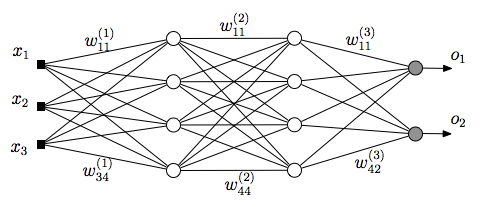
\includegraphics[scale=0.5]{img/MLP}
    \caption{Paveikslėlio pavyzdys}
    \label{img:mlp}
\end{figure}


\appendix{Eksperimentinio palyginimo rezultatai}

% tablesgenerator.com - converts calculators (e.g. excel) tables to LaTeX
\begin{table}[H]\footnotesize
  \centering
  \caption{Lentelės pavyzdys}
  {\begin{tabular}{|l|c|c|} \hline
    Algoritmas & $\bar{x}$ & $\sigma^{2}$ \\
    \hline
    Algoritmas A  & 1.6335    & 0.5584       \\
    Algoritmas B  & 1.7395    & 0.5647       \\
    \hline
  \end{tabular}}
  \label{tab:table example}
\end{table}

\end{document}
